% To build feynmf files, run 'make' once then do: mf '\mode=localfont; input $name'
\chapter{Theoretical Framework}
\label{chap:bg-theory}

\chapterquote{I am now convinced that theoretical physics is actually philosophy.}
{Max Born}

\section{Quantum Chromodynamics}
Quantum chromodynamics (\QCD) is the non-Abelian \SUgroup{3} gauge theory of the strong interaction.
Initially, it appears similar to \QED, with the single electric charge replaced by three conserved ``colour'' charges; there are, however, important differences between the two.

In the \QED Lagrangian, \EquationRef{eq:bg-theory:qed}, the electron carries one unit of charge, $-e$, the positron carries one unit of anti-charge $+e$ and the force is mediated by a massless photon.

\begin{gather}
  \label{eq:bg-theory:qed}
  \Lagrangian_{\QED} = \bar{\psi} \left(i \gamma^{\mu}  \partial_{\mu} -m \right) \psi - e \bar{\psi} \gamma^{\mu} A_{ \mu} \psi - \frac{1}{4}F_{\mu\nu}F^{\mu\nu}
  \intertext{where for a photon field $A_{\mu}$,}
  F_{\mu\nu} = \partial_{\mu} A_{\nu} - \partial_{\nu} A_{\mu} \nonumber
\end{gather}

Similarly, in the \QCD Lagrangian, \EquationRef{eq:bg-theory:qcd}, the quarks carry colour charge, $r, g, b$, anti-quarks carry anti-charge, $\bar{r}, \bar{g}, \bar{b}$ and the force is mediated by massless gluons.
As this is an exact \SUgroup{3} symmetry, the strong interaction is invariant under rotations in
colour space.

\begin{gather}
  \label{eq:bg-theory:qcd}
  \Lagrangian_{\QCD} = \bar{\psi}_{q,a} \left(i \gamma^{\mu}  \partial_{\mu} \delta_{ab} - m \delta_{ab} \right) \psi_{q,b} - \gQCD G^A_{\mu} \left( \bar{\psi}_{q,a} \gamma^{\mu} T^{ab}_A \psi_{q,b} \right) - \frac{1}{4}F^A_{\mu\nu}F_A^{\mu\nu}
  \intertext{where for a gluon field $G^A_{\mu}$,}
  F^A_{\mu\nu} = \partial_{\mu} G^A_{\nu} - \partial_{\nu} G^A_{\mu} - \gQCD f_{ABC} G^B_{\mu} G^C_{\nu} \nonumber
\end{gather}

In \EquationRef{eq:bg-theory:qcd}, the $\gamma^{\mu}$ are the Dirac $\gamma$-matrices and repeated indices are summed over, following the Einstein summation convention.
The $\psi$ are quark-field spinors for a quark of flavour $q$ and mass $m_q$, with a colour-index $a$ that runs from $a = 1$ to $N_c = 3$; quarks form the
fundamental representation of the \SUgroup{3} colour group.
The $G^A$ correspond to the gluon fields, with $A$ running from $1$ to $N_c^2-1 = 8$; there are eight types of gluon, forming the adjoint representation of the \SUgroup{3} colour group.
The $T^{ab}_A$ are eight $3 \times 3$ matrices, which form the generators of the \SUgroup{3} group, corresponding to the fact that the interaction between
a gluon and a quark rotates the quark in colour space.
Finally, \gQCD is the \QCD coupling constant and $F^A_{\mu\nu}$ the field tensor, where $f_{ABC}$ are the structure functions of the \SUgroup{3}.

In \QED, photons are electrically neutral and hence do not carry the charge of the EM interaction.
In contrast, gluons do carry colour charge, one unit of colour and one of anti-colour, so gluon self-interactions are to be expected.
Considering only the quark and gluon interaction terms the following simplified model of the \QCD Lagrangian can be obtained:

\begin{equation}
  \label{eq:bg-theory:qcd_simplified}
  \Lagrangian_{\QCD} = ``\qqbar" + ``G^{2}" + \gQCD``\qqbar G" + \gQCD``G^{3}" + \gQCD^{2}``G^{4}"
\end{equation}

Here, the $q$ correspond to quarks and the $G$ to gluons, with each term representing an allowed interaction or propagator within \QCD; the $G^3$ and $G^4$ terms represent triple and quartic gluon vertices.
The non-abelian $G^A_{\mu\nu}$ term in the Lagrangian, which gives rise to these terms, is thus the major reason for the greater complexity of \QCD in comparison to \QED.
As a result of gluon self-interactions, a \QCD process contains more diagrams at a given order than would be true for \QED.

\section{Asymptotic Freedom}
The interactions permitted by the \QCD Lagrangian mean that a quark or a gluon can emit a gluon, while gluons can make quark or gluon loops.
Analogously to \QED, these interactions are governed by a coupling constant, with $\alphaS = \frac{\gQCD^2}{4\pi}$.

Just as is the case with electric charge screening in \QED, the sum of the infinite series of higher order diagrams is equivalent to a single diagram with a ``running'' coupling constant.
However, in contrast to \QED, \alphaS \emph{decreases} with increasing \Qsquared, as can be seen in \EquationRef{eq:bg-theory:running_alpha_S}, resulting in ``anti-screening'' of colour charge.

\begin{gather}
  \label{eq:bg-theory:running_alpha_S}
  \alphaS\left(\Qsquared\right) \simeq \frac{\alphaS\left(Q_0^2\right)}{1 + B \alphaS\left(Q_0^2\right) \ln\left({\frac{\Qsquared}{Q_0^2}}\right)}
  \intertext{where for $N_c$ colours and $N_f$ quark flavours, the constant, $B$, is given by}
  B = \frac{11N_c - 2N_f}{12\pi} \nonumber
\end{gather}

At high \Qsquared, or equivalently at small distances, the effect of these higher order interactions can be conceptualised as spreading out the colour charge of an object into a ``colour cloud''.
A test charge inside the colour cloud will experience a smaller force than if it were a large distance away.
At small distances, therefore, quarks interact through colour fields of reduced strength and asymptotically behave like free particles. This phenomenon is known as asymptotic freedom and allows perturbation theory to be used in this region, permitting high precision tests, similar to those possible in \QED~\cite{Martin:2009:Nuclear}.

\section{Colour Confinement}
It is believed, although not yet proven, that all observable free particles must be colourless.
This is known as the colour confinement hypothesis: only colour singlet states can exist as free particles.
Consequently quarks are never observed in isolation but only in bound states as colourless hadrons.
Any energy injected into a hadron does not separate the quarks, but goes into creating \qqbar pairs and hence further hadrons.

\begin{figure}[htpb]
  \subfloat[Field lines arising from a \QED dipole]{
    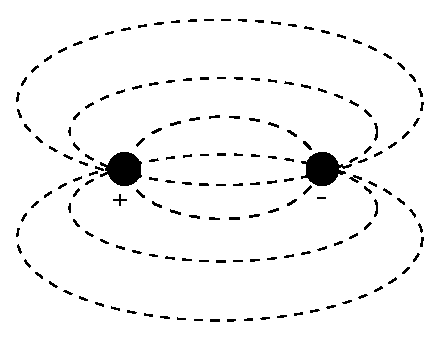
\includegraphics[width=\tinyfigwidth]{chapters/bg-theory/QEDDipoles.eps}
    \label{fig:bg-theory:qeddipole}}
  \qquad
  \subfloat[Field lines arising from a \QCD dipole]{
    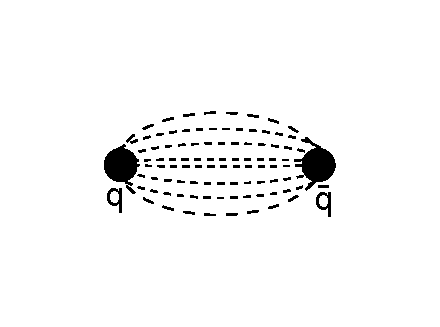
\includegraphics[width=\tinyfigwidth]{chapters/bg-theory/QCDTube.eps}
    \label{fig:bg-theory:qcddipole}}
  \caption{A comparison of the fields between \QED (electric) and \QCD (colour) dipoles: \protect\subref{fig:bg-theory:qeddipole} the electric field surrounding two opposite electric charges and \protect\subref{fig:bg-theory:qcddipole} the colour field surrounding a \qqbar pair  are shown. In comparison to the \QED case, the lines of force in \QCD are compressed. As the \qqbar separation, $r$, is increased, the \xs{al} area of the \QCD ``flux tube'' remains constant.}
  \label{fig:bg-theory:qedqcddipoles}
\end{figure}

Gluon self-interactions provide a plausible means by which colour confinement could arise.
When two coloured objects separate, the exchange of virtual gluons ``squeezes'' the lines of force between them so that they are closer together than in the \QED case and a ``flux tube'' of interacting gluons is formed (see \FigureRef{fig:bg-theory:qedqcddipoles}).
As the distance, $r$, between them increases, the \xs area of this tube remains approximately constant.
Since the number of field lines depends only on the colour of the sources, the field strength in the tube must also remain constant, while the field energy grows in proportion to the volume of the tube.
This means that the energy of the \qqbar system increases linearly with separation and hence that it would require an infinite amount of energy to fully separate two coloured objects~\cite{Gottfried:1986:concepts}.

\section{Evolution Equations}
\subsection{Deep Inelastic Scattering and the Quark-Parton Model}
The process in which the lepton from an \ep collision interacts with a quark from the proton is known as deep inelastic scattering (DIS).
If the interacting quark carries a fraction, $x$ of the proton's 4-momentum, $p$, then the \xs for this process is given by
%%The process in which the lepton from an \ep collision interacts with
%%a quark from the proton is known as deep inelastic scattering (DIS).

%%\begin{figure}[htpb]
%%  \parbox{100mm}{
%%    \vspace*{5mm}
%%    \unitlength=1mm
%%    \begin{fmffile}{dis}
%%      \begin{fmfgraph*}(100,50)
%%        \fmfleft{ip,il}
%%        \fmfright{oq1,oq2,d1,oq3,d2,d3,ol}
%%        \fmf{fermion}{ip,vp}
%%        \fmf{fermion,label=q $(xp)$}{vp,vq}
%%        \fmf{fermion,label=q $(p')$}{vq,oq3}
%%        \fmf{phantom}{ip,vp}
%%        \fmf{fermion}{vp,oq1}
%%        \fmf{fermion}{vp,oq2}
%%        \fmf{photon,tension=0.9,label=$\gamma / Z^{0} / W^{\pm} (q)$}{vl,vq}
%%        \fmf{fermion}{il,vl,ol}
%%        \fmf{phantom}{il,vl}
%%        \fmfblob{.15w}{vp}
%%        \fmfdot{vq,vl}
%%        \fmffreeze
%%        \fmfi{plain}{vpath (__ip,__vp) shifted (thick*(0,2))}
%%        \fmfi{plain}{vpath (__ip,__vp) shifted (thick*(1,-2))}
%%        \fmflabel{P ($p$)}{ip}
%%        \fmflabel{$e^{\pm}$ ($k$)}{il}
%%        \fmflabel{lepton}{ol}
%%        \fmflabel{proton remnant}{oq1}
%%      \end{fmfgraph*}
%%    \end{fmffile}
%%    \vspace*{5mm}
%%  }
%%  \caption{\ep deep inelastic scattering (DIS), mediated by a gauge boson}
%%  \label{fig:bg-theory:dis}
%%\end{figure}

%%As can be seen from \FigureRef{fig:bg-theory:dis}, the interacting quark
%%carries a fraction, $x$ of the proton's 4-momentum, $p$. The \xs for this
%%process is given by

\begin{align}
  \difDouble{\sigma}{x}{\Qsquared} &= \frac{4\pi\alpha^2}{Q^4} \left[ \left( 1 - y - \frac{m_p^2 y^2}{Q^2} \right) \frac{\F{2}}{x} + y^2 \F{1} \right] \\
  \intertext{or, in the high energy limit, where \Qsquared $\gg m_p^2y^2$} \nonumber \\
  &= \frac{4\pi\alpha^2}{Q^4} \left[ (1 - y) \frac{\F{2}}{x} + y^2 \F{1} \right]
  \label{eq:bg-theory:dsigmadQsquaredDIS}
\end{align}

%\begin{equation}
%\begin{split}
%  \dif{\sigma}{y} &= \frac{1}{8\pi}\frac{e^4 q_i^2}{Q^4} \hat{s} \left[ 1 + \left(1 - y\right)^2 \right] \\
%                  &= \frac{2\pi\alpha^2}{Q^4} q_i^2 \hat{s} \left[ 1 + \left(1 - y\right)^2 \right]
%  \label{eq:bg-theory:dsigmadQsquaredDIS}
%\end{split}
%\end{equation}
%\noindent where $\hat{s} = xs$ is the centre-of-mass energy of the interaction,
%$Q^2 = -q^2$ is related to the momentum transfer between the quark and the
%electron, $q_i = \pm 2/3, \pm 1/3$ is the electric charge of the struck quark
%and $y = \frac{q \cdot p}{k \cdot p}$ is the fraction of the electron's energy
%transferred to the proton in the proton's rest frame.

\noindent where $Q^2 = -q^2$ is related to the momentum transfer between the quark and the electron, $y = \frac{p_{p} \cdot q}{p_{p} \cdot p_{e}}$ is the fraction of the electron's energy transferred to the proton in the proton's rest frame, $m_p$ is the proton mass and \F{1} and \F{2} are, respectively, the pure magnetic and the electromagnetic proton structure functions, which describe the momentum distribution of the quarks within the proton.

In 1969, Bjorken proposed that the \F{1} and \F{2} structure functions should exhibit scaling behaviour in the deep inelastic limit, $\Qsquared \rightarrow \infty$ while $x$ stays finite~\cite{Bjorken:1969:scaling}.
Initially, this prediction, that the structure functions should be approximately independent of \Qsquared, was experimentally verified; more detailed investigation eventually showed the choice of $x$ with which the measurement was made to be serendipitous: at low $x$, \F{2} rises with increasing \Qsquared, while at high $x$, \F{2} falls with increasing \Qsquared.
It is nevertheless true that the structure functions depend more strongly on $x$, a kinematic quantity, than on \Qsquared, related to the energy of the collision.
In addition, it is observed that \F{1} and \F{2} are not independent, but satisfy the Callan-Gross relation:
%Since increasing energy
%provides for an improvement in spatial resolution, this scaling implies that the
%structure functions are independent of the absolute resolution scale, indicative
%of point-like substructure.

\begin{equation}
  F_2(x) = 2 x F_1(x)
\end{equation}

By analogy with \emu scattering, the differential \xs for elastic scattering between an electron and a quark with electric charge, $q_i = \pm 2/3, \pm 1/3$, and carrying a fraction, $x$, of the proton's 4-momentum, can be expressed as

\begin{equation}
\begin{split}
  \dif{\sigma}{\Qsquared} &= \frac{2\pi\alpha^2q_i^2}{Q^4} \left[ 1 + \left(1 - y\right)^2 \right] \\
  &= \frac{4\pi\alpha^2q_i^2}{Q^4} \left[ (1 - y) + \frac{y^2}{2} \right]
  \label{eq:bg-theory:dsigmadQsquared}
\end{split}
\end{equation}

In the proton, the fraction of quarks having $x$ in the range between $x_0$ and $x_0+\delta x$ is $\PDFq(x_0, \Qsquared)\delta x$ where $\PDFq$ is the parton distribution function (PDF) for the quark concerned.
Taking the distribution of quark momenta in this way, the \xs for scattering from a particular quark type within the proton is

\begin{equation}
  \dif{\sigma}{\Qsquared} \bigg|_{x \rightarrow x + \delta x} = \frac{4\pi\alpha^2}{Q^4} \left[ (1 -  y) + \frac{y^2}{2} \right] q_i^2 \PDFq_i( x, \Qsquared ) \delta x
\end{equation}

\noindent summing over all quarks and anti-quarks in the proton, since the gauge boson interacts equally with both, gives the expression

\begin{equation}
  \difDouble{\sigma}{\Qsquared}{x} = \frac{4\pi\alpha^2}{Q^4} \left[ (1 -  y) + \frac{y^2}{2} \right] \sum_i q_i^2 \PDFq_i(x, \Qsquared)
  \label{eq:bg-theory:dsigmadQsquareddxPDFs}
\end{equation}

Comparing \EquationRef{eq:bg-theory:dsigmadQsquareddxPDFs} and \EquationRef{eq:bg-theory:dsigmadQsquaredDIS} yields the parton model prediction
for the proton structure functions:

\begin{equation}
  \F{2} = 2x\F{1} = \sum_i \overbrace{x\PDFq_i(x, \Qsquared)}^{quark} + \overbrace{x\overline{\PDFq_i}(x, \Qsquared)}^{anti-quark}
  \label{eq:bg-theory:F2}
\end{equation}

In the proton, quarks, anti-quarks and gluons each have non-zero PDFs.
At present the \PDFq cannot be analytically calculated within \QCD: perturbation theory cannot be used due to the large coupling constant. The evolution of the PDFs with $x$ and $\Qsquared$, however, can be determined and tested experimentally.

\subsection{QCD Compton Scattering and Boson-Gluon Fusion}
\begin{figure}[htpb]
\begin{center}
  \parbox{99.9mm}{
    \vspace*{5mm}
    \unitlength=1mm
    \begin{fmffile}{qcdcompton}
      \begin{fmfgraph*}(100,50)
         \fmfleft{iq,ip}
         \fmfright{og,oq}
         \fmf{photon,label=$\gamma (q)$}{ip,v1}
         \fmf{fermion,label=$q_1 (yp)$}{iq,v2}
         \fmf{fermion,label=$q (xp)$}{v2,v1}
         \fmf{fermion,label=$q_2$}{v1,oq}
         \fmf{gluon,label=$g$}{v2,og}
      \end{fmfgraph*}
    \end{fmffile}
    \vspace*{5mm}
  }
  \caption{\QCD Compton scattering (\yqgq).}
  \label{fig:bg-theory:qcdcompton}
\end{center}
\end{figure}

In the \QCD Compton process (\FigureRef{fig:bg-theory:qcdcompton}), it can be shown that:

\begin{equation}
  \hat{\sigma}(\gamma q \rightarrow g q) \, = \, \int\limits_{\mu^2}^{\hat{s}/4} \mathrm{d}\pTsq \, \dif{\sigma}{\pTsq}
                                         \, = \, e_i^2 \sigma_0 \frac{\alphaS}{2\pi} \int\limits_{\mu^2}^{\hat{s}/4} \frac{\mathrm{d}\pTsq}{\pTsq} \, P_{qq}(z)
\end{equation}

\noindent where $\sigma_0 = \frac{4\pi^2\alpha}{\hat{s}}$ is the $\gamma^*p$ total \xs, \pT is the transverse momentum of the outgoing quark (see \SectionRef{sec:bg-theory:coordinates}), $\mu^2$ is an infrared cut-off to prevent divergences as $\pTsq \rightarrow 0$ and $P_{qq}(z) = \frac{4}{3}\left(\frac{1+z^2}{1-z}\right)$ is the probability of a quark emitting a gluon and so becoming a quark with momentum reduced by a fraction $z$.
Considering pure \QED and leading order \QCD diagrams gives:

\begin{equation}
\label{eq:bg-theory:qcdcompton}
\begin{split}
  \frac{\F{2}}{x} \bigg|_{\gamma^*q \rightarrow q (g)} &=
  \left|
  \parbox{17mm}{
    \begin{fmffile}{discompton1}
    \begin{fmfgraph*}(40,20)
      \fmfpen{thin}
      \fmfleft{iq,ip}
      \fmfright{oq}
      \fmf{photon}{ip,v1}
      \fmf{plain}{iq,v1,oq}
    \end{fmfgraph*}
    \end{fmffile}
  }
  \right|^2
  +
  \left|
  \parbox{17mm}{
    \begin{fmffile}{discompton2}
    \begin{fmfgraph*}(40,20)
      \fmfpen{thin}
      \fmfleft{iq,ip}
      \fmfright{og,oq,dummy}
      \fmf{photon}{ip,v1}
      \fmf{phantom}{iq,v1,oq}
      \fmf{plain,tension=0.1}{iq,v2,v1,oq}
      \fmffreeze
      \fmf{gluon}{v2,og}
    \end{fmfgraph*}
    \end{fmffile}
  }
  +
  \parbox{17mm}{
    \begin{fmffile}{discompton3}
    \begin{fmfgraph*}(40,20)
      \fmfpen{thin}
      \fmfleft{iq,ip}
      \fmfright{og,oq,dummy}
      \fmf{photon}{ip,v2}
      \fmf{phantom}{iq,v2,oq}
      \fmf{plain,tension=0.1}{iq,v2,v1,oq}
      \fmffreeze
      \fmf{gluon}{v1,og}
    \end{fmfgraph*}
    \end{fmffile}
  }
  \right|^2 \\
  &= \sum_q e_q^2 \int\limits_x^1 \frac{\mathrm{d}y}{y} \PDFq(y,\Qsquared) \left[ \delta \left( 1 - \frac{x}{y} \right) + \frac{\alphaS}{2\pi} P_{qq}\left(\frac{x}{y}\right)\ln\left({\frac{\Qsquared}{\mu^2}}\right) \right]
\end{split}
\end{equation}

At this order in \QCD, boson-gluon fusion must also be considered, with a similar expansion:

\begin{equation}
\label{eq:bg-theory:bgf}
\begin{split}
  \frac{\F{2}}{x} \bigg|_{\gamma^*g \rightarrow q \bar{q}} &=
  \left|
  \parbox{17mm}{
    \begin{fmffile}{bgf1}
    \begin{fmfgraph*}(40,20)
      \fmfpen{thin}
      \fmfleft{ig,ip}
      \fmfright{oq1,oq2}
      \fmf{gluon}{ig,v1}
      \fmf{plain}{oq1,v1,v2,oq2}
      \fmf{photon}{ip,v2}
    \end{fmfgraph*}
    \end{fmffile}
  }
  +
  \parbox{17mm}{
    \begin{fmffile}{bgf2}
    \begin{fmfgraph*}(40,20)
      \fmfpen{thin}
      \fmfleft{ig,ip}
      \fmfright{oq1,oq2}
      \fmf{gluon}{ig,v1}
      \fmf{phantom}{oq1,v1,v2,oq2}
      \fmf{photon}{ip,v2}
      \fmffreeze
      \fmf{plain}{oq1,v2,v1,oq2}
    \end{fmfgraph*}
    \end{fmffile}
  }
  \right|^2 \\
  &= \sum_q e_q^2 \int\limits_x^1 \frac{\mathrm{d}y}{y} \PDFg(y,\Qsquared) \frac{\alphaS}{2\pi} P_{gq}\left(\frac{x}{y}\right)\ln\left({\frac{\Qsquared}{\mu^2}}\right)
\end{split}
\end{equation}

\noindent where \PDFg is the gluon PDF in the proton and $P_{qg}(z) = \frac{1}{2}\left( z^2 + (1-z)^2 \right)$ is the probability that a gluon splits into a \qqbar pair.
Two further splitting functions are possible: $P_{gq}(z) = \frac{4}{3}\left( \frac{1 + (1-z)^2}{z} \right)$ is the probability that a quark emits a gluon which carries away a fraction $z$ of its momentum, and $P_{gg}(z) = 6\left( \frac{1-z}{z} + \frac{z}{1-z} + z(1-z) \right)$ is the probability that a gluon splits into two gluons; in each case these are unregulated probabilities, which contain singularities at $z=0$ or $z=1$.
Combining these results allows equations governing the evolution of the structure functions to be obtained.

\begin{align}
  \dif{\PDFq(x,\Qsquared)}{\ln{\Qsquared}} &= \frac{\alphaS}{2\pi} \int\limits_x^1 \frac{\mathrm{d}y}{y} \left( \PDFq(y,\Qsquared) P_{qq}\left(\frac{x}{y}\right) + \PDFg(y,\Qsquared) P_{qg}\left(\frac{x}{y}\right) \right) \label{eq:bg-theory:DGLAP1} \\
  \dif{\PDFg(x,\Qsquared)}{\ln{\Qsquared}} &= \frac{\alphaS}{2\pi} \int\limits_x^1 \frac{\mathrm{d}y}{y} \left( \sum_i \PDFq_i(y,\Qsquared) P_{gq}\left(\frac{x}{y}\right) + \PDFg(y,\Qsquared) P_{gg}\left(\frac{x}{y}\right) \right) \label{eq:bg-theory:DGLAP2}
\end{align}

\EquationsRef{eq:bg-theory:DGLAP1}{eq:bg-theory:DGLAP2} comprise the Dokshitzer-Gribov-Lipatov-Altarelli-Parisi (DGLAP) equations of parton evolution~\cite{Gribov:1972:DGLAP,Altarelli:1977:DGLAP,Dokshitzer:1977:DGLAP,Collins:1989:DGLAP}.
As shown here they are leading order in \alphaS but they have long been used at next-to-leading order and have recently been calculated at next-to-next-to-leading order~\cite{Moch:2004:threeLoop,Vogt:2004:threeLoop}.
Although derived by considering deep inelastic scattering, these equations describe the partonic structure of the proton and are applicable more generally.

\section{\QCD Factorisation}
\label{sec:bg-theory:qcd_factorisation}
At higher orders, the DGLAP equations become a summation over a series of integrals, each one similar in form to Equations~\ref{eq:bg-theory:DGLAP1} and~\ref{eq:bg-theory:DGLAP2}.
Within the context of DIS, initial state radiation means that the momentum of the parton at the point when it interacts with the photon can differ from its momentum when it was extracted from the proton.
Mostly, such momentum modifying emissions are collinear with the parton and are often considered as altering the structure of the proton rather than forming part of the calculation of the parton-photon interaction.
The separation between these two categories is defined using a factorisation scale, $\mu_F$.
Emissions with \pT above $\mu_F$ are included in the calculation, while emissions with lower \pT are accounted for in the proton PDFs.
This process, known as \QCD factorisation, separates the long-distance components (PDFs), which are universal, from the short-distance hard scattering, which is process dependent.

Additionally, due to the running of \alphaS as shown in \EquationRef{eq:bg-theory:running_alpha_S}, a choice must be made about the value of $Q$ at which \alphaS is evaluated.
This value, known as the renormalisation scale, $\mu_R$, is usually chosen to be of the order of a typical momentum transfer in the process being considered.

\begin{equation}
  \sigma_{\mathrm{jet}} = \sum_a \sum_b \overbrace{ \vphantom{\frac{Q^2}{\mu_R^2}} \PDF{a} \left( x_1, \mu_F^2 \right) \PDF{b} \left( x_2, \mu_F^2 \right) }^{PDFs}
    \overbrace{ \hat{\sigma}_{a,b} \left( p_{\Pproton1}, p_{\Pproton2}, \alphaS \left(\mu_R^2\right), \frac{Q^2}{\mu_F^2}, \frac{Q^2}{\mu_R^2} \right) }^{Hard~scatter}
    \label{eq:bg-theory:QCDfactorisation}
\end{equation}

\EquationRef{eq:bg-theory:QCDfactorisation} demonstrates how \QCD factorisation can be applied to proton-proton collisions.
Here the factorisation scale, $\mu_F$, is used in the evolution of the PDFs and fragmentation while the renormalisation scale, $\mu_R$, is connected to the momentum transfer at which the integration of \QCD equations stops.
$Q^2$ is a hard scale that characterises the parton-parton interaction while \PDF{a} and \PDF{b} are the PDFs of the interacting protons: typically jet measurements use $\mu_F = \mu_R = Q$.
Since the perturbation series is an asymptotic expansion, there is a limit to the precision with which any theoretical quantity can be calculated.
Independently varying the renormalisation and factorisation scales away from their chosen values, usually by factors of two, provides an indication of the
uncertainties on theoretical predictions.

\section{Hadronisation and Jets}
Perturbative QCD calculations may have coloured partons in the final state, but, due to colour confinement, only the colourless hadrons deriving from them are observed experimentally.

Consider a quark and anti-quark produced in, for example, an \Pelectron\Ppositron annihilation.
Initially, as the quarks separate, the interaction between them can be modelled by imagining a colour flux tube formed between them.
As the separation increases, so does the energy stored in this flux tube and hence the probability of \QCD radiation, which will be predominantly shallow-angled with respect to the originating parton.
Thus, one parton can radiate gluons, which will in turn radiate \qqbar pairs and so on, with each new parton nearly collinear with its parent.
This process, known as parton showering, produces partons of successively lower energy until, at some point, the interactions exit the region in which perturbative \QCD is valid.

Additionally, the coloured partons produced during this showering process must combine in bound states to form colourless hadrons.
This is known as hadronisation and results in collimated sprays of colourless particles, known as jets; the first evidence of jets arising from quarks was obtained in \Ppositron\Pelectron $\rightarrow$ \qqbar events at the SPEAR collider in 1975~\cite{Hanson:1975:jetstructure}.
Both hadronisation and the parton shower are inherently non-perturbative and must, therefore, be described using phenomenological models.

\section{Jets at Hadron Colliders}
\label{sec:bg-theory:jets_in_hadron_colliders}
Jets are unavoidable in hadron colliders, where the \QCD $2 \rightarrow 2$ scattering of partons is the dominant hard process.
This simple picture is complicated by higher order \QCD interactions, particularly hard gluon radiation, as well as by soft \QCD effects that have to be described using empirical models.

It is fundamentally impossible to examine the properties of partons: they are not physical objects but propagators, and their representation may vary according to, for instance, the \MC generator used.
Jets, on the other hand, are well-defined objects that, although not the same as partons, provide us with a window through which to investigate them.

Through looking at jets, \QCD can be studied by measuring parameters such as \alphaS or the top-quark mass.
\QCD calculations and phenomenological \MC models can be tested by measuring jet \xs{s}, providing constraints for future PDF fits.
The \QCD evolution equations can be tested by looking at rapidity gaps in \dijet systems, while jet substructure techniques provide a possible means of
identifying new physics.
Reconstructing decaying massive particles and constraining the structure of the proton both rely on accurate jet measurements.

\section{Co-ordinates at Hadron Colliders}
\label{sec:bg-theory:coordinates}
In a hadron collider the centre-of-mass frame of the hadrons is not usually the same as the centre-of-mass frame of the interacting partons.
Energy and angular separations are not invariant under Lorentz boosts and, for a detector constructed in the hadronic centre-of-mass frame, particles will appear more collimated or dispersed depending on their boost.

It is therefore important, particularly when dealing with jets which are produced with a range of different boosts, to choose variables which are longitudinally Lorentz invariant with which to classify events.
Rapidity, \rap, is a spatial coordinate describing the angle of a particle relative to the beam axis.
At a hadron collider, particle production is roughly constant as a function of \rap.

\begin{equation}
  \rap = \frac{1}{2}\ln{\frac{E+p_z}{E-p_z}}
\end{equation}

Pseudorapidity, \pseudorap, is a well-defined function of the polar angle, $\theta$ which also provides a close approximation to rapidity; they are identical in the limit of massless particles.

\begin{equation}
  \pseudorap = -\ln \left( \tan{\frac{\theta}{2}} \right) = \frac{1}{2}\ln{\frac{p+p_z}{p-p_z}}
\end{equation}

For angles approximately perpendicular to the beam axis, $\theta = \pi/2 + \delta\theta$, it can be seen that distance in \pseudorap is equivalent to distance in $\theta$:

\begin{equation}
\begin{split}
  \DeltaEta &= -\ln \left( \tan{\frac{\theta_1}{2}} \right) + \ln \left( \tan{\frac{\theta_2}{2}} \right) \\
            &= -\ln \left( 1 + 2\frac{\delta\theta_1}{2} \right) + \ln \left( 1 + 2\frac{\delta\theta_2}{2} \right) \\
            &= -\ln \left( 1 + \delta\theta_1 \right) + \ln \left( 1 + \delta\theta_2 \right) \\
            &= \delta\theta_2 - \delta\theta_1 = \Delta\theta
\end{split}
\end{equation}

Physical momenta are usually measured in terms of transverse momentum, \pT
\begin{equation}
  \pT = \sqrt{ p_x^2 + p_y^2 }
\end{equation}

Polar angle in the transverse plane, $\phi$, is left unchanged by longitudinal boosts.

\section{Luminosity at Hadron Colliders}
\label{sec:bg-theory:luminosity}
The luminosity of a proton-proton collider can be expressed as

\begin{equation}
  \luminosity = \frac{R_{inel}}{\sigma_{inel}}
\end{equation}

where $R_{inel}$ is the rate at which inelastic collisions occur and $\sigma_{inel}$ the corresponding \xs.
For a collider operating at a revolution frequency, $f_r$ with $n_b$ bunches crossing per revolution, this can be expressed as

\begin{equation}
  \label{eq:bg-theory:luminosity_vis}
  \luminosity = \frac{\mu n_b f_r}{\sigma_{inel}} = \frac{\mu^{vis} n_b f_r}{\epsilon \sigma_{inel}} = \frac{\mu^{vis} n_b f_r}{\sigma_{vis}}
\end{equation}

\noindent where $\mu$ is the average number of inelastic interactions per bunch crossing, $\epsilon$ the efficiency for one inelastic collision to satisfy the event selection criteria for a visible process of interest and, for the chosen process, $\sigma^{vis}$ and $\mu^{vis}$ are the \xs and number of inelastic interactions per bunch crossing respectively.

The absolute luminosity, \luminosity, can be inferred from measured accelerator parameters, using the equation

\begin{equation}
  \label{eq:bg-theory:vdMscan}
  \luminosity = \frac{n_b f_r n_1 n_2}{2 \pi \Sigmax \Sigmay}
\end{equation}

\noindent where $n_1$ and $n_2$ are the numbers of particles in the two colliding bunches, while \Sigmax and \Sigmay characterise the widths of the beam profile in the horizontal and vertical directions respectively.
\Sigmax and \Sigmay are usually measured using van der Meer scans, in which the observed event rate is recorded while scanning the opposing beams across each other in the horizontal and vertical directions.

The luminosity determined using \EquationRef{eq:bg-theory:vdMscan}, together with the measured value of $\mu_{vis}$ can then be used to calculate $\sigma_{vis}$ using \EquationRef{eq:bg-theory:luminosity_vis}, without relying on knowledge of the total inelastic \xs or measurements of detector inefficiencies.

\section{Jet Algorithms}
To first order defining a jet is simple: it relies on identifying a coherent stream of particles originating at the interaction point.
However, it is neither feasible nor repeatable to do this manually on an event-by-event basis: a well-defined jet algorithm is needed.

A jet algorithm is a fully specified set of rules for projecting information from a large number of hadron-like objects onto a small number of parton-like
objects.
These rules should work at all levels in order to allow fair and straightforward comparisons between data and theory.
A jet algorithm should be able to take final-state particles from \MC, partons produced in a fixed order \pQCD calculation or detector level objects such as calorimeter towers or tracks as input, while its output should be order independent and minimally dependent on hadronisation and detector effects that are often only understood empirically.

Jets need to be theoretically well-behaved, in other words, they must be invariant under minor modifications of their constituents.
Specifically, adding a soft parton should not change the jet clustering results, a property known as infrared safety, while the identified jets should similarly remain unchanged if one parton is replaced by a collinear pair of partons, usually termed collinear safety.
Without these requirements, real-virtual cancellations in next-to-leading order (NLO) and next-to-next-to-leading order (NNLO) \QCD calculations are not possible, producing divergent results.
This leads to large uncertainties, removing much of the benefit obtained from calculating NLO quantities in the first place.
From an experimental perspective, since detectors can resolve neither the full collinear nor the full infrared structure of an event, it is important that jet definitions are invariant in these limits.

The construction of a jet is unavoidably ambiguous in at least two ways.
The first of these is the decision over which particles will be combined to form a jet: in other words the choice of which jet algorithm and associated parameters to use.
The second is the question of how to recombine the momenta of these particles into a single four-vector to be assigned to the identified jet.

When taken together, these different elements determine the particular jets that will be identified in an event, although, in general, physical results, such as particle discovery, masses or couplings, should be independent of the choice of jet definition.
There are two main classes of jet algorithm: cone algorithms and sequential recombination algorithms.

\subsection{Cone Algorithms}
Cone algorithms have historically been important in hadron collider experiments, due to their apparent conceptual simplicity and fast execution time.
The basic idea underlying algorithms of this type is to cluster objects together based on their proximity in \yphi space. Given a cone with centroid, $C$, and radius, $R$, a typical cone algorithm will take all objects $i$ satisfying

\begin{equation}
  \sqrt{ \left(y^i-y^C\right)^2 + \left(\phi^i-\phi^C\right)^2 } \leq R
\end{equation}

\noindent and use them to determine the properties of the cone:

\begin{equation}
\begin{split}
  & \quad p^C = \left(E^C,\mathbf{p}^C \right) = \sum_i \left( E^i, p_x^i, p_y^i, p_z^i \right), \\
  & \overline{y^C} = \frac{1}{2} \ln{ \frac{E^C+p_z^C}{E^C-p_z^C} }, \qquad \overline{\phi^C} = \tan^{-1}{ \left( \frac{p_y^C}{p_x^C} \right) }
\end{split}
\end{equation}

\noindent If $y^C = \overline{y^C}$ and $\phi^C = \overline{\phi^C}$ then the sum of the momenta of all particles inside the cone points in the same direction as the cone centroid and the cone is identified as ``stable''.
If the cone is not stable, the clustering step is repeated using the new centroid.
This process is repeated iteratively until all identified cones are stable.

Cone algorithms of this sort usually rely on an initial step in which a subset of the available objects are identified as ``seeds'': the initial centroids used to start the clustering step.
Usually, all objects above some \pT threshold are selected as seeds: something which is inherently infrared unsafe, as the particular distribution of soft objects or electronic noise will affect which objects are above this threshold.

Additionally, cone algorithms need a procedure to deal with the case in which two stable cones overlap: usually this comes in the form of a parameter which determines whether to merge the two cones or to split them along a plane perpendicular to the line joining their centroids.
This split/merge parameter is commonly expressed as a function of the percentage of \pT overlap between the constituents of the two cones.

Except in cases of overlap, cone algorithms produce regular, circular jets.
This regularity of shape facilitates the comparison and calibration of jets.
Unfortunately, with the exception of the SISCone algorithm~\cite{Salam:2007:SISCone}, cone algorithms are, in general, infrared and collinear unsafe, making them a poor choice for comparisons between data and theory.

\subsection{Recombination Algorithms}
\label{bg-theory:recombination_algorithms}
As an approximation, the development of a jet can be thought of as a consequence of repeated $1 \rightarrow 2$ branching of quarks and gluons within \QCD.
Sequential recombination algorithms aim to work their way backwards through these branches, repeatedly combining pairs of particles into a single one.

Clearly, an algorithm using this approach must define which pair of particles to combine at each step and how to determine when the end of the process has been reached.
Obviously at each step, the best particles to combine are those which are in some way ``closest'' to one another; a metric to determine the distance
between each pair of particles must therefore be defined:

\begin{equation}
  d_{ij}^2 = \min\left( \pTrecomb{i}, \, \pTrecomb{j} \right) \frac{\DeltaR_{ij}^2}{R^2}, \qquad d_{iB} = \pTrecomb{i}
\end{equation}

\noindent where $\DeltaR_{ij}^2 = \left(y^i-y^j\right)^2 + \left(\phi^i-\phi^j\right)^2$, $d_{ij}$ represents the distance between particles $i$ and $j$  and $d_{iB}$ the distance between particle $i$ and the beam remnant.
The different types of recombination algorithm can be distinguished by the value of $p$ that they use

\begin{equation}
  p = \left\{
  \begin{array}{c l}
    1 & \quad \text{\kt algorithm~\cite{Catani:1991:kt,Catani:1993:kt}}\\
    0 & \quad \text{\CA algorithm~\cite{Dokshitzer:1997:CambridgeAachen,Wobisch:1998:CambridgeAachen}}\\
    -1 & \quad \text{\akt algorithm~\cite{Cacciari:2008:antikt}}
  \end{array} \right.
\end{equation}

In each case, given a minimal interjet separation, $R$, the algorithm proceeds by calculating $d_{i(j,B)}$ between each pair of objects and finds the smallest of these.
If this is from the set $d_{ij}$ then objects $i$ and $j$ are combined; if it is from the set $d_{iB}$ then $i$ is identified as a jet and removed from
the list of objects.
This process is repeated iteratively until there are no objects left.
Historically, this has been computationally intensive, but recently an efficient implementation has been developed and is available through the \fastjet software package~\cite{Cacciari:2005:fastjet,Cacciari:2012:fastjet}.

Sequential recombination algorithms of this type guarantee that all jets will be separated by a distance of at least $R$ on a \yphi cylinder.
The absolute number of jets is not infrared safe, as soft jets can be identified near the beam remnant, but, if a \pT threshold is instituted, the number of jets above the threshold represents an infrared safe quantity.

The \CA algorithm is the simplest recombination algorithm, relying only on distance weighting.
Because of this, it is sensitive to the distribution of soft objects, often producing irregularly shaped jets.
Because the \CA algorithm has a clustering hierarchy which is dependent on angle, it is possible to view a specific jet on a range of angular scales, a feature which is commonly used in studies of jet substructure.

The \kt algorithm forms clusters from pairs of low \pT objects.
By combining objects in this way, it is inherently collinear safe, proactively including soft \QCD radiation. This means that \kt jets can have irregular shapes which are complicated to deal with experimentally, particularly when attempting to correct for the effects of underlying event or pileup.

The \akt algorithm forms clusters from pairs of high-\pT particles, disfavouring clustering between pairs of soft objects.
Unlike \kt and \CA, reversing the order of clustering in \akt cannot be usefully related to sequential branching in \QCD, essentially \akt proceeds by agglomerating soft material into an existing hard subjet, rather than by first constructing the soft subjet and then recombining it with the hard subjet.
Most pairwise clusterings will involve at least one hard object and such an object will therefore tend to accumulate all softer objects within $R$ of its centroid.
This results in \akt jets having a roughly circular shape with radius $\simeq R$, allowing for easy experimental calibration.
This feature has led to \akt being adopted as the default jet algorithm used by the \ATLAS and \CMS experiments.

A comparison between different jet algorithms can be seen in \FigureRef{fig:bg-theory:jet_algorithms}.
Here the jets produced by \kt, \CA, \akt and SISCone are shown, using the same input distribution of particles and the same $R$-parameter in each case.
The two highest \pT jets in the event, here shown in green and red, are essentially identical in each case, although the precise details of which particles are combined are different in each case.
Additionally, there is some variation in the ordering of the lower \pT jets.
The circular shapes of the \akt jets and the irregular outline of the \kt jets are particularly notable.

\begin{figure}[htpb]
  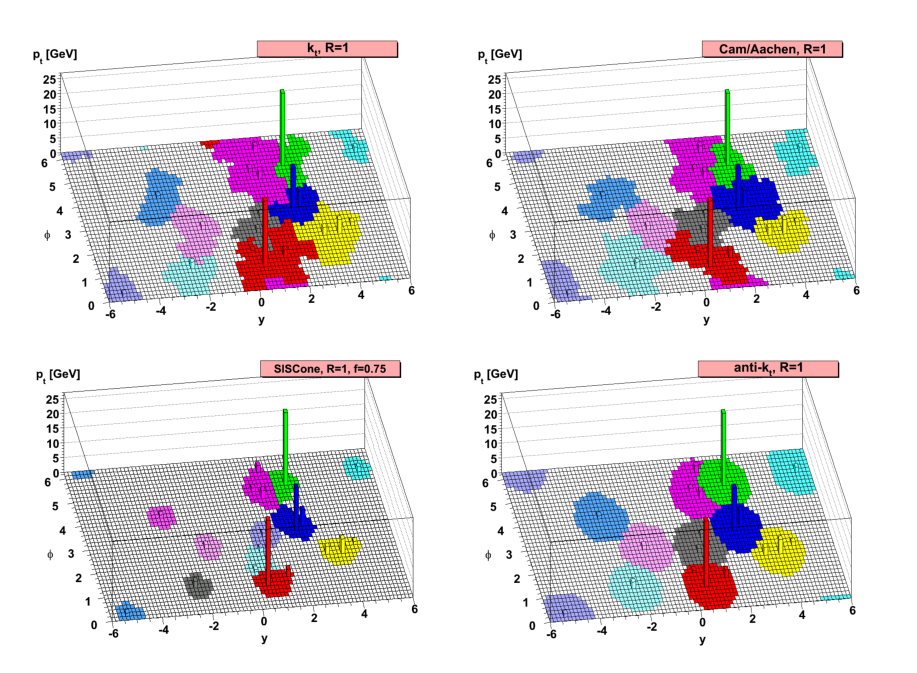
\includegraphics[width=\largefigwidth]{chapters/bg-theory/JetAlgComparison.eps}
  \caption{A sample \Herwig (see \SectionRef{sec:bg-theory:MC:Herwig}) generated parton level event, overlaid with random soft particles, clustered with four different jet algorithms, illustrating the shapes and sizes of the resulting hard jets. For \kt and \CA the detailed shapes are partially determined by the specific set of soft particles used, and would change if these were to be modified~\cite{Cacciari:2005:fastjet,Cacciari:2012:fastjet}.}
  \label{fig:bg-theory:jet_algorithms}
\end{figure}

\section{\MC Generators}
\label{sec:bg-theory:MC_generators}
The \MC method refers to any procedure that makes use of random numbers and probabilistic statistics to solve problems.
\MC methods are used extensively in numerical analysis and simulation of natural phenomena.
In the context of particle physics, \MC generators are used to produce theoretical simulations of real events.
Often a variety of different programs are used: feasibly one program could generate a hard process while another evolves it through a parton
shower algorithm and a third hadronises the coloured products of the shower.
Different \MC generators often simulate different physics models, using different matrix elements, PDFs, evolution equations, parton showers or
hadronisation models.
Because of this, comparing a variety of \MC models to data provides a test of the compatibility of different theories with experimental results.
The simulation of physics events in \ATLAS is carried out in two steps:

\begin{itemize}
  \item \textbf{Event generation}: Theoretical and phenomenological models are used to simulate the physics processes which result from proton-proton collisions, producing particle level information as an output.
  \item \textbf{Detector simulation}: These final-state particles are passed through a full simulation of the \ATLAS detector~\cite{ATLAS:2010:simulation} that is based on \GEANT~\cite{Agostinelli:2003:GEANT4} and aims to reproduce the behaviour of particles as seen in test-beam studies.
\end{itemize}

After a given \MC generator has produced particle level predictions which have been passed through the \ATLAS simulation, the events are treated in the same way as data: in particular, jets are reconstructed and calibrated using the reconstruction chain discussed in \SectionRef{sec:analysis-tools:jet_reconstruction}.

\subsection{\Pythia}
\label{sec:bg-theory:MC:Pythia}
The \Pythia~\cite{Sjostrand:2006:pythia6.4} \MC generator implements leading-order matrix elements from perturbative \QCD for $2\rightarrow2$ processes, followed by \pT-ordered parton showers, calculated in the leading-logarithm approximation and finally the Lund string model for hadronisation.
The underlying event in \Pythia consists mainly of multiple-parton interactions interleaved with the initial state parton shower.
Samples used in \ATLAS are generated using the \ATLAS Minimum Bias Tune 1 (AMBT1) set of parameters~\cite{ATLAS-CONF-2010-031}, in which the non-diffractive model is tuned to \ATLAS measurements of charged particle production at $\rootS = \unit{900}{\GeV}$ and $\rootS = \unit{7}{\TeV}$.
The AMBT1 tune uses the Martin-Roberts-Stirling-Thorne (MRST) LO* PDFs~\cite{Sherstnev:2008:LOMC,Martin:2009:lhcpartons}.

\Pythia~6.423 events produced with the \Perugia~2011~\cite{Skands:2010:perugia} set of tuned parameters are also used.
These parameters have been tuned to reproduce the jet shape and hadronic event shape spectra seen in \LEP and \Tevatron data.

\subsection{\Herwig}
\label{sec:bg-theory:MC:Herwig}
The \Herwig~\cite{Corcella:2001:Herwig} generator uses identical leading order matrix elements to \Pythia, but applies an angular-ordered parton shower and a clustering hadronisation model.
For the underlying event, \Herwig~6 is linked to \Jimmy~\cite{Butterworth:1996:JIMMY} to provide multiple partonic interactions.
\Herwigpp~\cite{Bahr:2008:Herwigpp}, the latest version of \Herwig, directly implements a \Jimmy-like approach to the underlying event.
The \Herwigpp event samples are generated using the MRST LO* PDF set with the \LHC Underlying Event~7-2 (LHC-UE7-2) tune for the underlying event~\cite{Gieseke:2011:Herwigpp}.

\subsection{\Alpgen}
\label{sec:bg-theory:MC:Alpgen}
The \Alpgen~\cite{Mangano:2003:Alpgen} \MC generator provides leading order matrix elements with up to six partons in the final state.
The \Alpgen samples are generated using the CTEQ6L1 PDF set, from the Coordinated Theoretical-Experimental Project~\cite{Pumplin:2002:CTEQ6L1} and are then passed through \Herwig and \Jimmy (see \SectionRef{sec:bg-theory:MC:Herwig}) to provide parton showering, hadronisation and multiple partonic interactions with the \ATLAS Underlying Event Tune 1 (AUET1) set of parameters~\cite{ATLAS-PHYS-PUB-2010-014}.

\subsection{\Powheg}
\label{sec:bg-theory:MC:Powheg}
\Powheg~\cite{Nason:2004:NLOMC,Frixione:2007:NLOPowheg,Alioli:2010:NLOPowheg} is a generator capable of simulating next-to-leading order inclusive jet and \dijet production.
\Powheg allows the use of either \Pythia or \Herwig to shower the partons, hadronise them, and model the underlying event.
The advantage over the standard $2\rightarrow2$ matrix elements that are provided in \Pythia and \Herwig, is that the emission of a third hard parton is calculated at matrix element level, allowing observables that are dependent on the third jet to be calculated more accurately.

In the \Powheg algorithm, the genesis of each event comes from a \QCD $2\rightarrow2$ partonic scatter. The renormalisation and factorisation scales are then both set to be equal to the transverse momentum of the outgoing partons, before the hardest partonic emission in the event is generated using the Martin-Stirling-Thorne-Watt (MSTW) 2008 NLO PDFs.
Once the hardest partonic emission is simulated, the events can be evolved to the hadron level.
The fact that \Powheg has a full parton shower interface ensures that, unlike in the case of fixed order NLO calculations, accurate predictions can be produced for multijet final states without the need to independently estimate soft corrections and their associated uncertainties.

\subsection{\NLOjetpp}
\label{sec:bg-theory:NLOjetpp}
\NLOjetpp is not a \MC generator, but rather a C++ program for explicitly determining leading and next-to-leading order \xs{s}.
It uses a modified form of the Catani-Seymour dipole subtraction method to calculate a variety of \QCD processes in proton-proton collisions.
Currently, \NLOjetpp is able to compute $n$-jet \xs{s} at next-to-leading order for $n \leq 3$ as well as four-jet \xs{s} at leading order.

In order to provide results which are comparable with data, final distributions produced by \NLOjetpp have to be corrected for the effects of hadronisation.
Usually this is done on a bin-by-bin basis: final distributions are produced using \NLOjetpp and separately using a leading-order \MC such as \Pythia.
The \Pythia distributions are produced both at parton level, taking only the final state partons in the event, and at hadron level, once these partons have passed through the relevant hadronisation model.
The ratio between these two distributions is then applied to the \NLOjetpp distribution as a correction for the effects of hadronisation.
Several different leading order \MC{s} are used in order to allow an estimation of the uncertainty in physics modelling arising from this procedure.

\subsection{\HEJ}
\label{sec:bg-theory:MC:HEJ}
High Energy Jets (\HEJ) is a \MC generator aiming to simulate production of multiple jets at a hadron collider.
It is based on the BFKL kernel, implementing an all-order resummation of the perturbative terms which dominate the production of well-separated multijet events.
This calculation is made in the limit of infinite rapidity separation between all partons produced in the event and is therefore most suited to events in which the most forward and most backward jets are widely separated.

The $2 \rightarrow n$ matrix elements are studied for $n \ge 2$ in the Multi-Regge kinematic limit in which scattering amplitudes are dominated by $t$-channel gluon exchange~\cite{Andersen:2009:Factorisation} and each of the successively emitted, rapidity-ordered gluons has a similar momentum to the previous ones.
In this limit, the perturbative terms which describe multiple gluon emissions can be factorised, with the final scattering amplitude depending only on the transverse momenta of the emitted gluons.

This method approximates real emissions at all orders, also including virtual emissions in a way that ensures that any soft divergences from the virtual corrections cancel with those from gluon emissions.
This results in a regularised matrix element at all orders in \alphaS, with contributions coming from any number, greater than two, of hard jets. The jet rates have been fully matched to tree-level accuracy up to a total of four jets.

As the centre-of-mass energy increases, the hard radiative corrections that \HEJ was developed to describe become increasingly important; particularly when considering \dijet systems with a large invariant mass or a large rapidity difference between the jets.

At present, \HEJ is only capable of producing parton level predictions as it does not yet have proper parton shower matching. However, since it is not a
fixed order calculation, the number of partons produced is variable, and relatively large in comparison to standard fixed order generators.
Accordingly, in order to provide meaningful results, the partons produced as output by \HEJ must be clustered into jets and corrected for soft effects in the same manner as described for \NLOjetpp in \SectionRef{sec:bg-theory:NLOjetpp}.
